\documentclass[12pt]{article}
\usepackage[]{fullpage}
\usepackage[]{graphicx}
\usepackage{booktabs}
\usepackage{colortbl}
\usepackage{adjustbox}
\usepackage{xcolor}
\usepackage{amsmath}
\title{Report}
\author{GP Team 2015}
\date{\today}
\begin{document}
\maketitle
\newpage
\tableofcontents
\newpage

\section{Introduction}
What is a graphic? How can we succinctly describe a graphic? And how can we create the graphic
that we have described? \\
 \\
  These are important questions for the field of statistical graphics.
One way to answer these questions is to develop a grammar . A good grammar will allow us to gain insight
into the composition of complicated graphics, and reveal unexpected connections between seemingly
different graphics. \\ \\
 A grammar provides a strong foundation for understanding a diverse range of graphics.
A grammar may also help guide us on what a well­formed or correct graphic looks like, but there will still
be many grammatically correct but nonsensical graphics.
\\ \\
 This is easy to see by analogy to the English
language: good grammar is just the first step in creating a good sentence. Grammar makes language
expressive. A language consisting of words and no grammar (statement = word) expresses only as many
ideas as there are words. By specifying how words are combined in statements, a grammar expands a
language's scope.
\\ \\
 In other hand grammar of graphics is a tool that enable us to concisely describe the
components of graphic. Such a grammar allow us to move beyond named graphics “scatterplot” and gain
insight into the deep structure that underlies statistical graphics . \\ The power of the grammar is illustrated with a selection of examples that explore different components and their interactions .

\newpage
\section{Literature review}
\subsection{Data Visualization}
\subsubsection{Definition}
Data visualization is the presentation of data in a pictorial or graphical format. For centuries, people have depended on visual representations such as charts and maps to understand information more easily and quickly. \\ \\
Because of the way the human brain processes information, it is faster for people to grasp the meaning of many data points when they are displayed in charts and graphs rather than poring over piles of spreadsheets or reading pages and pages of reports.
\\
\subsubsection{Data visualization importance}
Visualizations help people see things that were not obvious to them before. \\ \\
A spreadsheet cannot visually represent the information due to data presentation limitations, would spend hours searching among thousands of rows and columns of data with still no concrete answer about the relationship between two factors.
\\
\begin{figure}[h!]
\caption{The path of Napoleon's troops across the Russian Empire of Alexander I}
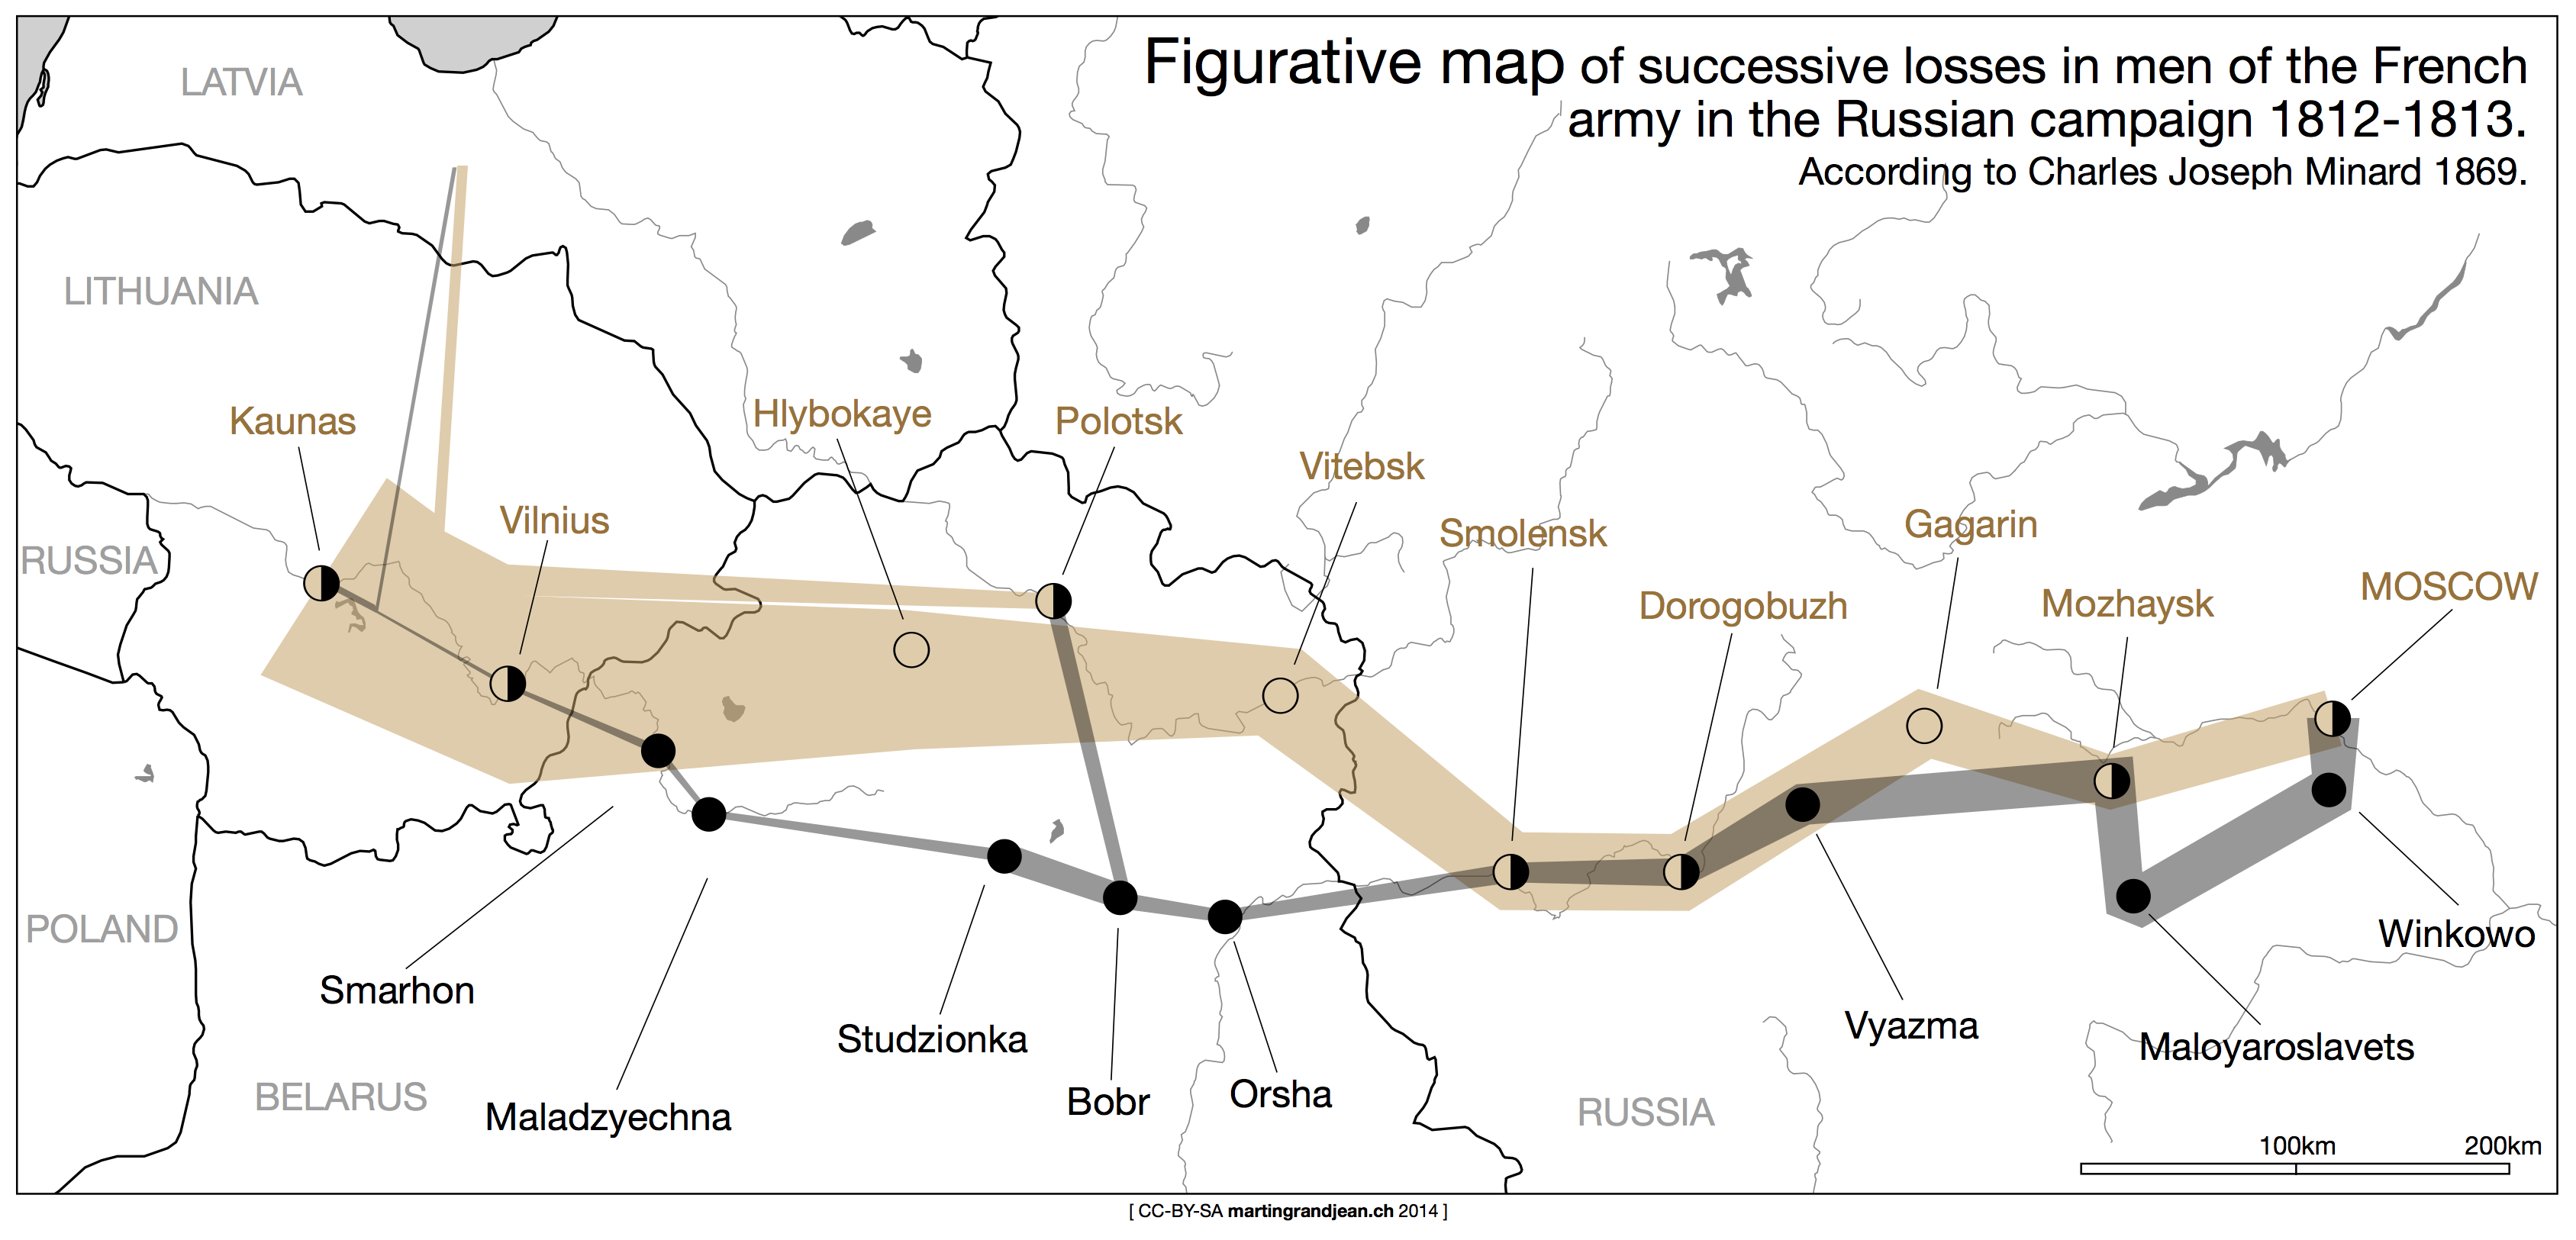
\includegraphics[width=\textwidth]{Minard2Geo2}

\end{figure}
\newpage
\section{Grammar of graphics}
\subsection{What is the meaning of Grammar?}
the whole system and structure of a language or of languages in general, usually taken as consisting of syntax and morphology (including inflections) and sometimes also phonology and semantics. \\
So if we think about the graphics as a language from the perspective of the grammar we should put in our minds those rules (grammar) that manage that manage these sentences or the components of the language (charts). \\
\subsection{What is the Grammar of Graphics?}
The regime of constructing the graphs depending on predefined rules, Hence 
The grammar of graphics takes us beyond a limited set of charts (words) to an almost unlimited world of graphical forms (statements).
\subsection{Grammar of graphics features}
\begin{itemize}
\item Orthogonal set of features describes all common charts, Virtually all uncommon charts.
\item Language is flexible enough to
\begin{itemize}
\item describe our known chart types
\item describe unknown chart types
\end{itemize}
\end{itemize}
\begin{figure}[h!]
\caption{Grammar of graphics layers}
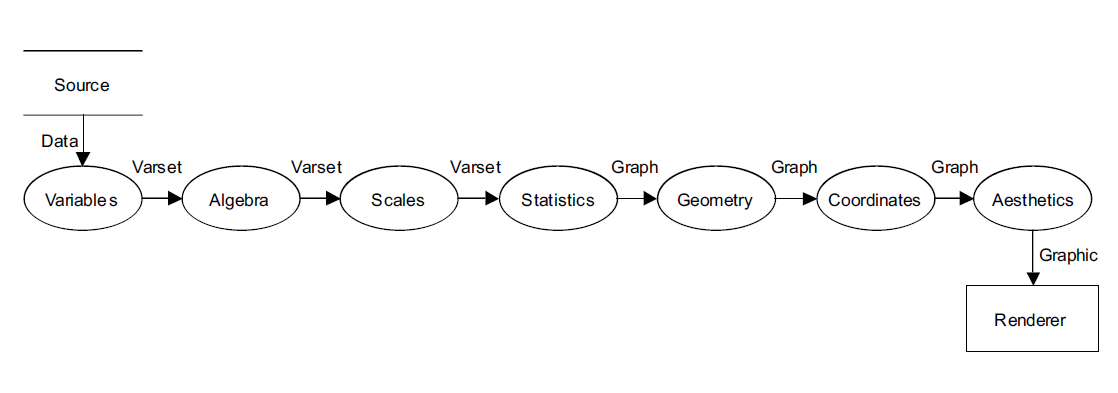
\includegraphics[width=\textwidth]{pre9}
\end{figure}
\newpage
\section{Comparative study among GoG libraries }
\begin{table}[!th]
\caption{Comparative Study}
\label{my-label}
\begin{adjustbox}{max width=450}
\begin{tabular}{|l|l|l|l|l|}
		\hline
		\rowcolor[HTML]{9B9B9B} 
		\multicolumn{1}{|c|}{\cellcolor[HTML]{9B9B9B}\textbf{Library}} & \multicolumn{1}{c|}{\cellcolor[HTML]{9B9B9B}\textbf{ggplot2}}                                                                                                                                                                                                                    & \multicolumn{1}{c|}{\cellcolor[HTML]{9B9B9B}\textbf{ggvis}}                                                                                                                                                                              & \multicolumn{1}{c|}{\cellcolor[HTML]{9B9B9B}\textbf{ggd3}}                             & \multicolumn{1}{c|}{\cellcolor[HTML]{9B9B9B}\textbf{vega}}                                                                             \\ \hline
		\textbf{Implementation}                                        & Fully Implemented                                                                                                                                                                                                                                                                & Fully Implemented                                                                                                                                                                                                                        & Partially Implemented                                                                  & \begin{tabular}[c]{@{}l@{}}Partially Implemented\\ GOG\end{tabular}                                                                    \\ \hline
		\textbf{Language}                                              & \multicolumn{1}{c|}{R}                                                                                                                                                                                                                                                           & \multicolumn{1}{c|}{R}                                                                                                                                                                                                                   & \multicolumn{1}{c|}{JavaScript}                                                       & \multicolumn{1}{c|}{JavaScript}                                                                                                       \\ \hline
		\textbf{Issue}                                                 & No interactivity.                                                                                                                                                                                                                                                                & Limited Interactivity                                                                                                                                                                                                                    & \begin{tabular}[c]{@{}l@{}}-Have fixed set of geoms.\\ -No interactivity.\end{tabular} & Set of static geometrics.                                                                                                              \\ \hline
		\textbf{Description}                                           & \begin{tabular}[c]{@{}l@{}}It takes care of many \\ of the fiddly details\\  that make plotting a\\  hassle (like drawing\\  legends) as well as \\ providing a powerful \\ model of graphics\\ that makes it easy to \\ produce complex \\ multi-layered graphics.\end{tabular} & \begin{tabular}[c]{@{}l@{}}-Declaratively describe\\ data graphics with a syntax \\ similar in spirit to ggplot2.\\ -Create rich interactive\\ graphics that you \\ can play with locally in \\ Rstudio or in your browser.\end{tabular} & Stop development                                                                       & \begin{tabular}[c]{@{}l@{}}Vega is a declarative\\  format for creating,\\  saving, and sharing \\ visualization designs.\end{tabular} \\ \hline
	\end{tabular}
	\end{adjustbox}
\end{table}
\section{Our Approach}
Design \& Implement a library that is based on Grammar of graphics to be the baseline of continuous contribution in the field of data visualization. \\
\begin{enumerate}
\item GoG library.
\begin{itemize}
\item built with javascript runs on Node.js environment
\end{itemize}
\item Application Layer.
\begin{itemize}
\item built on top of Electron.
\end{itemize}
\item Package Manager.
\begin{itemize}
\item which will manage application extensions and plugins.
\end{itemize}
\end{enumerate}

\section{Team members playrolls}
\subsection{Raafat Sobhy}
\begin{itemize}
\item List \& implement Coordinate systems
\begin{itemize}
\item Number line
­\item Cartesian coordinate system
\item Polar coordinate system
\item ­ Cylindrical and spherical coordinate systems
\item Homogeneous coordinate system
\end{itemize}
\end{itemize}
\subsection{Sherif Embarak}
\begin{itemize}
\item adding full documentation to all function
\item partial implementation for link, bin, region and summary functions
\item importing csv files to js objects
\end{itemize}
\subsection{Ahmed Fouad}
\begin{itemize}
\item List predefined figures in GoG book
\item implementing geometric components (point, line, circle)
\end{itemize}
\subsection{Yusuf Mohamed}
\begin{itemize}
\item {\Large Package Manager} for application layer.
\begin{itemize}
\item A cli utility tool which fetches \& removes plugins (extensible piece of code) from npm and places it in specific folder. once the application bootstraps it will check all the existing plugins in the folder to add them which will provide feature rich application.
\item why use a new directory for plugins?
\begin{itemize}
\item The idea behind using a new directory other than \texttt{node\_modules} is that the application will lookup plugins in it, and application shouldn't lookup plugins in the \texttt{node\_modules} folders, as it will be another problem to differentiate between plugins and other node modules.
So, the separation is needed to help the visualization application lookup plugins in a folders containing plugins only.
\end{itemize}
\item Works on all major platforms like Windows, Linux and Mac.
\item Took in consideration various plugin manager design like apm (\texttt{atom package manager}) and Brackets plugins.
\item why didn't we use apm or brackets plugin manager?
\begin{itemize}
\item APM : no documentation or how-to, limits the plugins to be hosted on github only.
\item Brackets : limits the developer with a specific structure and specific keywords to make his plugin up and running.
\end{itemize}
\item Usage
\begin{itemize}
\item Add Or Update a plugin.
\begin{equation*}
vispack \hspace{3} install \hspace{3} plugin\_name \nonumber
\end{equation*}
\item Remove a plugin
\begin{equation*}
vispack \hspace{3} remove \hspace{3} plugin\_name \nonumber
\end{equation*}
\end{itemize}

\end{itemize}
\item {\Large Application Layer}
\begin{itemize}
\item Made with electron formerly known as NW.js which is a cross platform application to distribute the application on all major platforms and photon kit for styling.
\item Interprocess communication \texttt{ipc} to coordinate activities among different program process (main process and rendering process) via sending and  receiving messages between the mentioned processes.
\end{itemize}
\end{itemize}
\begin{figure}[h!]
\caption{Prototype Design}
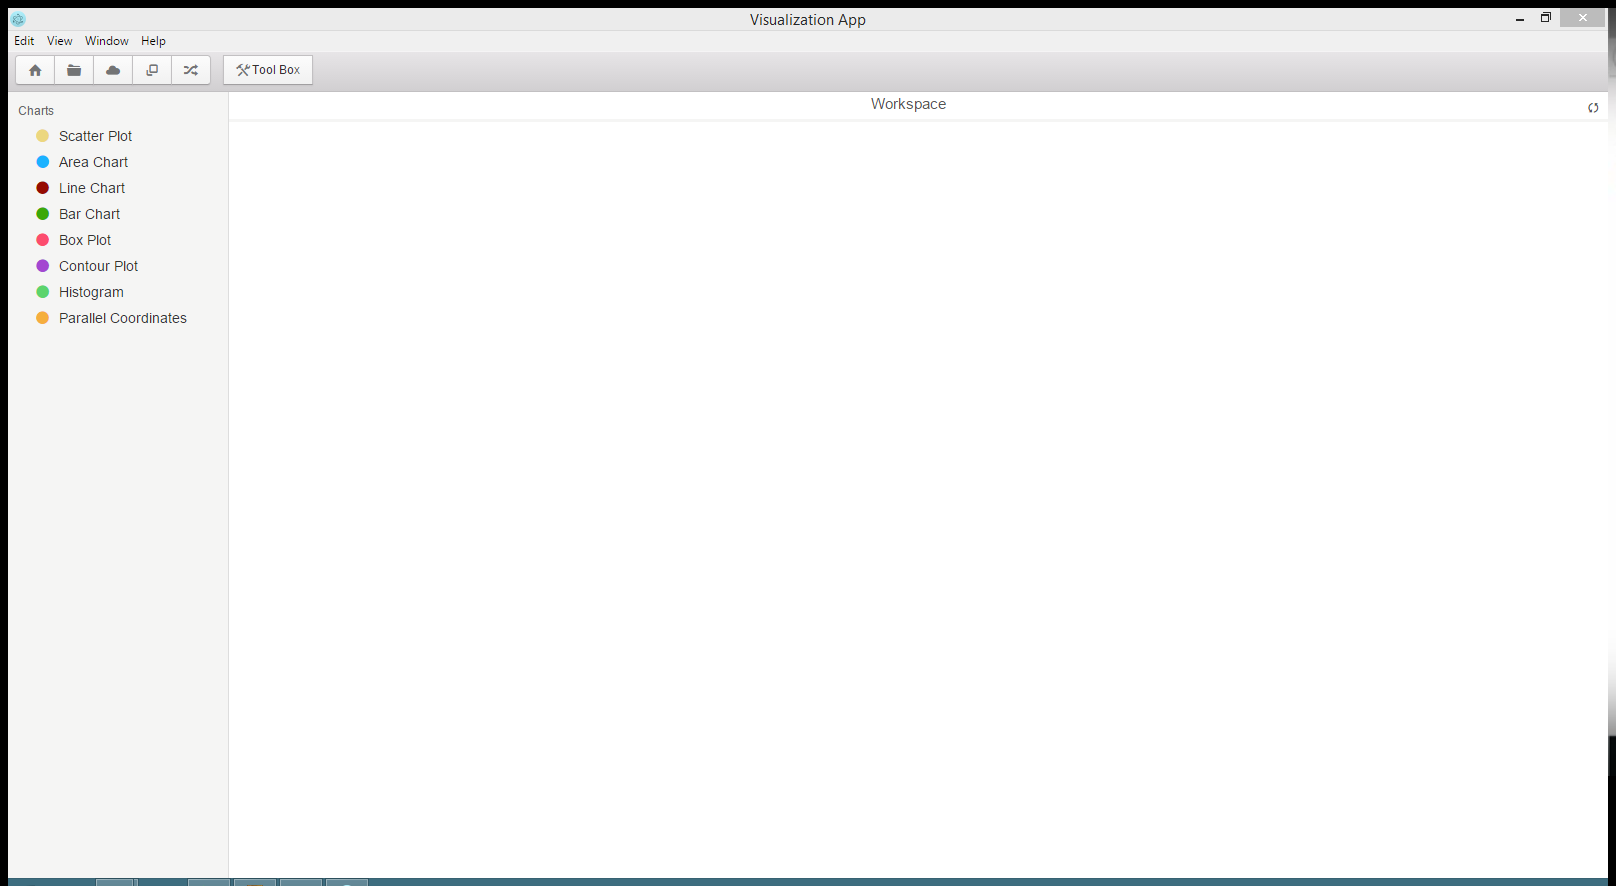
\includegraphics[width=\textwidth]{prototype}

\end{figure}

\section{Gantt Chart}
\begin{figure}[h!]
\caption{Gantt chart}
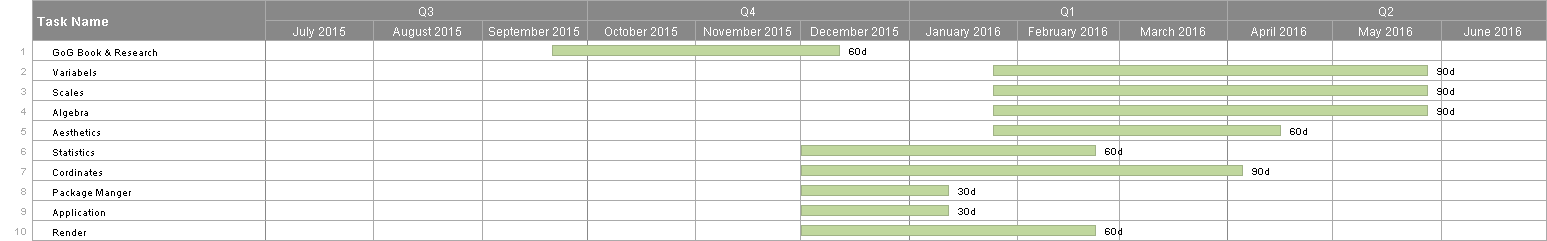
\includegraphics[width=\textwidth]{gantt}

\end{figure}

\section{Deliverable}
Partial implementation of GoG library which will make us able to generate the following charts
\begin{itemize}
\item Scatter Plot
\item Area Chart
\item Line Chart
\item Bar Chart
\item Histogram
\item Parallel Coordinates
\item Scatter Plot Matrix 
\end{itemize}


\begin{thebibliography}{10}
\bibitem VVega \texttt{http://vega.github.io/}
\bibitem gggplot2 \texttt{http://ggplot2.org/}
\bibitem gggvis \texttt{http://ggvis.rstudio.com/}
\bibitem gggd3 \texttt{http://benjh33.github.io/ggd3/}
\end{thebibliography} 
\end{document}
